
\chapter{Linear transformations}

\index{linear transformation}
\index{function}

A \textbf{linear transformation} is actually just another spin on matrix-vector
multiplication. It's also yet another way to view a matrix as a
\textit{function}. Back on p.~\pageref{matrixIsFunction}, I made the point that
instead of drawing numbers in a grid, you could view a matrix itself as a
function, where the input is an ordered pair (row and column numbers) and the
output is the element at that entry. In this chapter, we explore a deeper and
richer interpretation of a matrix as a \textit{different} sort of function.

\section{Transforming one vector into another}

Recall how matrix-vector multiplication works. We'll write it notationally as
$A \cdot \overrightarrow{\textbf{x}} = \overrightarrow{\textbf{y}}$, where
$\overrightarrow{\textbf{y}}$ is the result of the multiplication. Now we could
think about the operation like this:

\begin{compactitem}
\item $A$ is a ``function'' of sorts, which works on vectors to produce other
vectors.
\item $\overrightarrow{\textbf{x}}$ is the input vector we give to that
function.
\item $\overrightarrow{\textbf{y}}$ is the function's output (result).
\end{compactitem}

\index{machine}
We're thinking of $A$ as a long-lasting, reusable thing, whereas
$\overrightarrow{\textbf{x}}$ and $\overrightarrow{\textbf{y}}$ stand for the
temporary inputs \& outputs that we give to $A$ and compute on the fly. My
mental image is of $A$ as a machine, $\overrightarrow{\textbf{x}}$ as the raw
materials we might feed to the machine, and $\overrightarrow{\textbf{y}}$ as
the machine's completed work.

One natural question is: ``what is the domain, and the range, of this $A$
function?'' That depends on $A$'s dimensions. Suppose it's a $3\times 2$
matrix:

\vspace{-.15in}
\begin{align*}
\begin{bmatrix}
2 & 3 \\
1 & -4 \\
0 & 5 \\
\end{bmatrix} \cdot \textrm{\Large ?} = \textrm{\Large ?}
\end{align*}
\vspace{-.15in}

\index{domain}
\index{codomain}
We know from the rules of matrix-vector multiplication
(p.~\pageref{matVecRules}) that the first question mark has to be a
\textbf{2}-dimensional column vector, else the operation is impossible. And we
know that the output will be a \textbf{3}-dimensional column vector. This means
that the domain of the $A$ ``function'' is 2-d vectors and the codomain is 3-d
vectors. Most commonly, this is written as follows:

\vspace{-.15in}
\begin{align*}
A : \mathbb{R}^2 \rightarrow \mathbb{R}^3.
\end{align*}
\vspace{-.15in}

Remember from \textit{A Cool, Brisk Walk} that the $\mathbb{R}$ sign means
``the set of real numbers.'' When we say ``$\mathbb{R}^2$'' we're saying ``the
set of vectors with two real-numbered entries.'' And $\mathbb{R}^3$ is the set
of \textit{three}-dimensional real vectors, \textit{etc.}

Put all together, the purpose of our $A$ matrix is to map each two-dimensional
vector to a particular three-dimensional vector. For instance, it maps the 2-d
vector $[\ 2 \ \ 1\ ]$ to:

\vspace{-.15in}
\begin{align*}
\begin{bmatrix}
2 & 3 \\
1 & -4 \\
0 & 5 \\
\end{bmatrix} \cdot 
\begin{bmatrix}
2 \\ 1 \\
\end{bmatrix} =
\begin{bmatrix}
7 \\ -2 \\ 5 \\
\end{bmatrix}.
\end{align*}
\vspace{-.15in}

The particular vector it chooses seems kind of random so far, and indeed this
first example is just pulled from the air. Normally there will be some
``meaning'' to the transformation.

\index{linear map}

By the way, a linear transformation is sometimes called a \textbf{linear map}
because it performs this ``mapping'' operation, like a function does. The two
terms (linear transformation and linear map) are exact synonyms.

\subsection{Meaningful examples}

Before we go any further, let's at least show that this is useful. I'm going to
create a machine (matrix) $B$ (for ``Body,'' sort of) that transforms certain
4-dimensional vectors into 2-dimensional ones. Here it is:

\vspace{-.15in}
\begin{align*}
B = 
\begin{bmatrix}
12 & 1 & 0 & 0 \\
0 & 0 & 2.2 & 0 \\
\end{bmatrix}.
\end{align*}
\vspace{-.15in}

The kind of input this matrix/function is intended to act on a vector such as
$\overrightarrow{\textbf{stephen}}$, which is structured like this:

\vspace{-.3in} 
\begin{align*}
\begin{matrix*}[r]
\textrm{\small{height: whole feet}} \rightarrow \\
\textrm{\small{height: extra inches}} \rightarrow \\
\textrm{\small{weight: kilograms}} \rightarrow \\
\textrm{\small{shoe size}} \rightarrow \\
\end{matrix*}
\begin{bmatrix}
6 \\ 2 \\ 95.5 \\ 13 \\
\end{bmatrix}
\end{align*}
\vspace{-.15in}

This rather revealing vector contains some of my vital bodily stats. I'm 6'2"
tall, and hence don't fit on airplanes; I weigh too much at 95.5 kg; and I wear
an impossible-to-fit 13 shoe (13AAA, actually; blame my mom's side of the
family).

Now what happens when we feed this to the $B$ machine?

\vspace{-.15in}
\begin{align*}
B \cdot \overrightarrow{\textbf{stephen}} =
\begin{bmatrix}
12 & 1 & 0 & 0 \\
0 & 0 & 2.2 & 0 \\
\end{bmatrix} \cdot
\begin{bmatrix}
6 \\ 2 \\ 95.5 \\ 13 \\
\end{bmatrix} =
\begin{bmatrix}
74 \\ 210 \\
\end{bmatrix}
\begin{matrix*}[l]
\leftarrow \textrm{\small{height in inches}} \\
\leftarrow \textrm{\small{weight in pounds}} \\
\end{matrix*}
\end{align*}
\vspace{-.15in}

This matrix-vector multiplication produces a 2-element vector, since

\vspace{-.15in}
\begin{align*}
B : \mathbb{R}^4 \rightarrow \mathbb{R}^2.
\end{align*}
\vspace{-.15in}

The first element is my height in total inches, and the second element is my
weight in pounds. And it will do so for every person whose 4-dimensional vector
it's multiplied by. Interestingly, the shoe size of the input vector plays no
role in the value of the output vector, because there are zero elements at both
$B_{0,3}$ and $B_{1,3}$. And that's okay.

\smallskip
\index{BMI (body-mass index)}

By the way, you might think about expanding this example to calculate something
more complex like a BMI (body-mass index). After all, BMI is a straightforward
function of a person's weight and height\footnote{(Mine's about 27, which puts
me in the ``obese'' range I'm sorry to say.)}, as you might know:

\vspace{-.15in}
\begin{align*}
\textrm{BMI} = 703 \times \frac{\textrm{weights (lbs)}}{\textrm{height (in)}^2}.
\end{align*}
\vspace{-.15in}


However, it turns out this is \textit{impossible} to do with a linear
transformation. The reason is it's not linear! The only operations that can be
included in a linear transformation are dot products, because that's what
matrix-vector multiplication \textit{is}. So for each element of our output
vector, we can (1) take the elements of the input vector, (2) multiply each of
them by any constant we like, and (3) add up the results. The BMI formula, by
contrast, requires us to \textit{divide} one of our inputs by another, and in
fact requires us to \textit{square} that second input before dividing. These
are both decidedly non-linear operations that cannot be expressed with a
matrix.

This may seem limiting, and in a way it is, but keep in mind two things. First,
there are lots and lots and lots of common operations that \textit{are} linear,
and all of those come under our power in this book on linear algebra. Second,
when we do have linear operations, we can take advantage of all kinds of
computational simplifications and analytical tricks, so concentrating on the
linear case is most definitely worth our time.

\bigskip

\index{stock price}
Here's a second example. Suppose I have the following odd-looking matrix $S$
(for ``stocks,'' sort of):

\vspace{-.15in}
\begin{align*}
S =
\begin{bmatrix}
0 & 1 & 0 \\
0 & .69 & 0 \\
0 & 111.1 & 0 \\
0 & .88 & 0 \\
0 & 6.48 & 0 \\
0 & 17.37 & 0 \\
\end{bmatrix}
\end{align*}
\vspace{-.15in}

What does it do? Well, it's designed for us to feed it vectors representing
Wall Street stocks, like so:

\index{McDonald's}
\vspace{-.3in} 
\begin{align*}
\overrightarrow{\textbf{mcdonalds}} =
\begin{bmatrix}
1965 \\ 183.52 \\ 2606707 \\
\end{bmatrix}
\begin{matrix*}[l]
\leftarrow\textrm{\small{year founded}} \\
\leftarrow\textrm{\small{current share price}} \\
\leftarrow\textrm{\small{trading volume}} \\
\end{matrix*}
\end{align*}
\vspace{-.15in}

The result of multiplying $S$ by this kind of vector is to give us a
convenient list of the McDonald's current stock price in various currencies:

\vspace{-.3in} 
\begin{align*}
S \cdot \overrightarrow{\textbf{mcdonalds}} =
%\begin{bmatrix}
%0 & 1 & 0 \\
%0 & .69 & 0 \\
%0 & 111.1 & 0 \\
%0 & .88 & 0 \\
%0 & 6.48 & 0 \\
%0 & 17.37 & 0 \\
%\end{bmatrix} \cdot
%\begin{bmatrix}
%1965 \\ 183.52 \\ 2606707 \\
%\end{bmatrix} =
\begin{bmatrix}
183.52 \\ 126.93 \\ 20389.10 \\ 161.50 \\ 1189.21 \\ 3187.74 \\
\end{bmatrix}
\begin{matrix*}[l]
\leftarrow\textrm{\small{\EyesDollar \ (U.S. dollars)}} \\
\leftarrow\textrm{\small{\pounds \ (British pounds sterling)}} \\
\leftarrow\textrm{\small{\textyen \ (Japanese Yen)}} \\
\leftarrow\textrm{\small{\EURtm \ (Euros)}} \\
\leftarrow\textrm{\small{\textyen \ (Chinese Yuan)}} \\
\leftarrow\textrm{\small{\textpeso \ (Mexican Pesos)}} \\
\end{matrix*}
\end{align*}
\vspace{-.15in}

Again, the $S$ matrix is simply ignoring the information we don't care about,
and that's okay. It's still a function:

\vspace{-.15in}
\begin{align*}
S : \mathbb{R}^3 \rightarrow \mathbb{R}^6.
\end{align*}
\vspace{-.15in}


\section{Linear operators}

\index{square matrix}
\index{linear operator}

So every matrix gives us a linear transformation, no matter its shape. But if
the matrix is \textit{square}, we use a special name for the linear
transformation it carries out: a \textbf{linear operator}.

A matrix being square, of course, would imply that the input vectors and the
output vectors (or the domain and codomain, if you prefer) are the \textit{same
dimension}: the function will map vectors in $\mathbb{R}^3$ to other vectors in
$\mathbb{R}^3$, for instance, or from $\mathbb{R}^{81}$ to $\mathbb{R}^{81}$.

Let's restrict our attention for the moment to just two dimensions, and see
what effect certain $2\times 2$ linear operator matrices have on the vectors
they act upon.

\begin{figure}[hb]
\centering
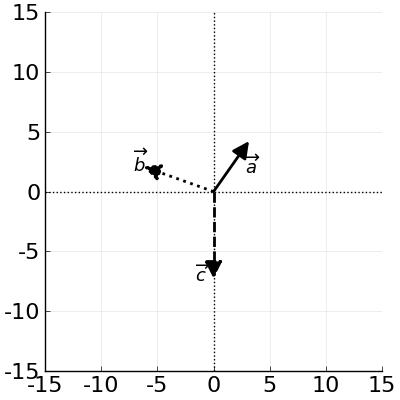
\includegraphics[width=0.44\textwidth]{preoperators.png}
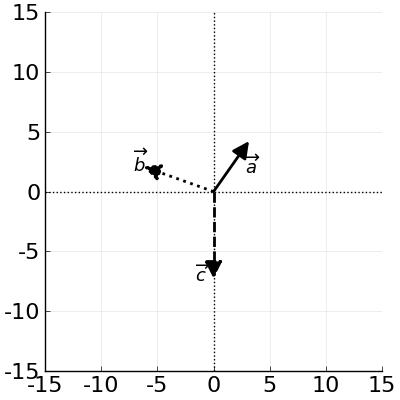
\includegraphics[width=0.44\textwidth]{preoperators.png}
\caption[.]{Three vectors, and their transformations under the super boring
linear operator {\scriptsize $\begin{bmatrix} 1 & 0 \\ 0 & 1 \\
\end{bmatrix}$.}}
\label{fig:identityOp}
\end{figure}

\index{identity matrix}

We'll have three guinea pig vectors, which are:
$\overrightarrow{\textbf{a}} = [\ 3\ \ 4\ ]$ (solid),
$\overrightarrow{\textbf{b}} = [\ -6\ \ 2\ ]$ (dotted), and
$\overrightarrow{\textbf{c}} = [\ 0\ \ -7\ ]$ (dashed). They're plotted in the
left half of Figure~\ref{fig:identityOp}. First, we'll try the identity matrix,
which you'll remember in two dimensions is simply:

\vspace{-.15in}
\begin{align*}
I_2 =
\begin{bmatrix}
1 & 0 \\
0 & 1 \\
\end{bmatrix}
\end{align*}
\vspace{-.15in}


Let's multiply our three guinea pigs by this matrix to transform them:

\vspace{-.15in}
\begin{align*}
I_2 \cdot \overrightarrow{\textbf{a}} &=
\begin{bmatrix}
1 & 0 \\
0 & 1 \\
\end{bmatrix} \cdot
\begin{bmatrix}
3 \\ 4 \\
\end{bmatrix} =
\begin{bmatrix}
3 \\ 4 \\
\end{bmatrix}.
\end{align*}

\vspace{-.15in}
\begin{align*}
I_2 \cdot \overrightarrow{\textbf{b}} &=
\begin{bmatrix}
1 & 0 \\
0 & 1 \\
\end{bmatrix} \cdot
\begin{bmatrix}
-6 \\ 2 \\
\end{bmatrix} =
\begin{bmatrix}
-6 \\ 2 \\
\end{bmatrix}.
\end{align*}

\vspace{-.15in}
\begin{align*}
I_2 \cdot \overrightarrow{\textbf{c}} &=
\begin{bmatrix}
1 & 0 \\
0 & 1 \\
\end{bmatrix} \cdot
\begin{bmatrix}
0 \\ -7 \\
\end{bmatrix} =
\begin{bmatrix}
0 \\ -7 \\
\end{bmatrix}.
\end{align*}
\vspace{-.15in}

The effect, you'll agree, is underwhelming. Double-check my math, and convince
yourself that \textit{the function of the identity matrix is to convert a
vector into itself!} This is why it's called the ``identity'' matrix, in fact.
The ``identity element'' of addition is 0, which means if you add anything to
zero, you get your number back as an answer. The identity element of
multiplication is 1, of course. And fun fact, the identity \textit{matrix} is
the matrix {\tiny $\begin{bmatrix} 1 & 0 \\ 0 & 1 \\ \end{bmatrix}$}.

The right half of Figure~\ref{fig:identityOp} illustrates this boring fact:
under the identity matrix's linear operator, all three vectors look exactly the
same after the transformation.

\medskip

K, let's shake things up a bit then. Let's try this operator:

\vspace{-.15in}
\begin{align*}
S_{v=2} =
\begin{bmatrix}
1 & 0 \\
0 & 2 \\
\end{bmatrix}.
\end{align*}
\vspace{-.15in}

I'll reveal why I chose $S_{v=2}$ as the name of this matrix in a moment.
Notice that it is the same as $I_2$ except for the 2 in the bottom-right
corner. What does it do when it maps vectors? Let's give it a shot:

\vspace{-.15in}
\begin{align*}
S_{v=2} \cdot \overrightarrow{\textbf{a}} &=
\begin{bmatrix}
1 & 0 \\
0 & 2 \\
\end{bmatrix} \cdot
\begin{bmatrix}
3 \\ 4 \\
\end{bmatrix} =
\begin{bmatrix}
3 \\ 8 \\
\end{bmatrix},
\end{align*}

\vspace{-.15in}
\begin{align*}
S_{v=2} \cdot \overrightarrow{\textbf{b}} &=
\begin{bmatrix}
1 & 0 \\
0 & 2 \\
\end{bmatrix} \cdot
\begin{bmatrix}
-6 \\ 2 \\
\end{bmatrix} =
\begin{bmatrix}
-6 \\ 4 \\
\end{bmatrix},
\end{align*}

\vspace{-.15in}
\begin{align*}
S_{v=2} \cdot \overrightarrow{\textbf{c}} &=
\begin{bmatrix}
1 & 0 \\
0 & 2 \\
\end{bmatrix} \cdot
\begin{bmatrix}
0 \\ -7 \\
\end{bmatrix} =
\begin{bmatrix}
0 \\ -14 \\
\end{bmatrix}.
\end{align*}
\vspace{-.15in}

\begin{figure}[ht]
\centering
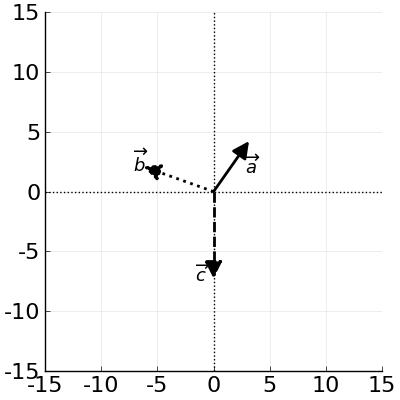
\includegraphics[width=0.44\textwidth]{preoperators.png}
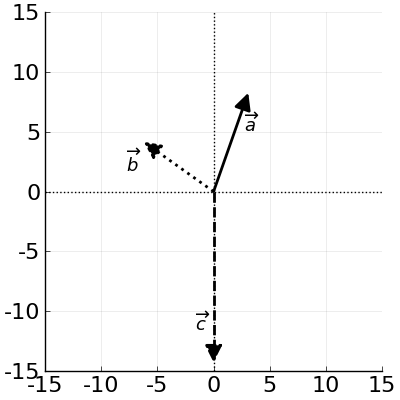
\includegraphics[width=0.44\textwidth]{vertstretchop.png}
\caption[.]{Three vectors, and their transformations under the slightly more
interesting linear operator 
{\scriptsize $\begin{bmatrix} 1 & 0 \\ 0 & 2 \\ \end{bmatrix}$.}}
\label{fig:vertstretchop}
\end{figure}

\index{stretching}
Can you see what it did in Figure~\ref{fig:vertstretchop}? It
\textit{stretched all the points vertically by a factor of 2.} In other words,
every vector is now pointing at a point twice as far from the $x$-axis. This is
why I chose the name $S_{v=2}$ -- it stands for ``\textbf{S}tretch
\textbf{v}ertically by a factor of \textbf{2}.''

\pagebreak

Playing on the same theme, we can try:

\vspace{-.15in}
\begin{align*}
S_{v=\frac{1}{2},h=2\frac{1}{2}} =
\begin{bmatrix}
2\frac{1}{2} & 0 \\
0 & \frac{1}{2} \\
\end{bmatrix}.
\end{align*}
\vspace{-.15in}

Let's see what this bad boy does to our vectors:

\vspace{-.15in}
\begin{align*}
S_{v=\frac{1}{2},h=2\frac{1}{2}} \cdot \overrightarrow{\textbf{a}} &=
\begin{bmatrix}
2\frac{1}{2} & 0 \\
0 & \frac{1}{2} \\
\end{bmatrix} \cdot
\begin{bmatrix}
3 \\ 4 \\
\end{bmatrix} =
\begin{bmatrix}
7\frac{1}{2} \\ 2 \\
\end{bmatrix},
\end{align*}

\vspace{-.15in}
\begin{align*}
S_{v=\frac{1}{2},h=2\frac{1}{2}} \cdot \overrightarrow{\textbf{b}} &=
\begin{bmatrix}
2\frac{1}{2} & 0 \\
0 & \frac{1}{2} \\
\end{bmatrix} \cdot
\begin{bmatrix}
-6 \\ 2 \\
\end{bmatrix} =
\begin{bmatrix}
-15 \\ 1 \\
\end{bmatrix}.
\end{align*}

\vspace{-.15in}
\begin{align*}
S_{v=\frac{1}{2},h=2\frac{1}{2}} \cdot \overrightarrow{\textbf{c}} &=
\begin{bmatrix}
2\frac{1}{2} & 0 \\
0 & \frac{1}{2} \\
\end{bmatrix} \cdot
\begin{bmatrix}
0 \\ -7 \\
\end{bmatrix} =
\begin{bmatrix}
0 \\ -3.5 \\
\end{bmatrix}.
\end{align*}
\vspace{-.15in}

\begin{figure}[ht]
\centering
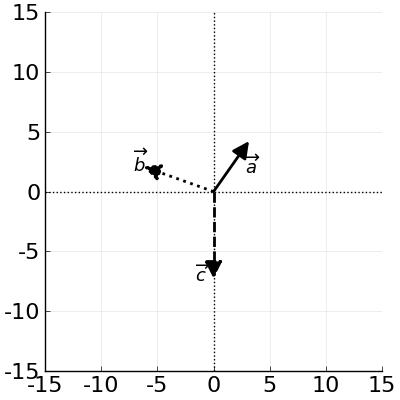
\includegraphics[width=0.44\textwidth]{preoperators.png}
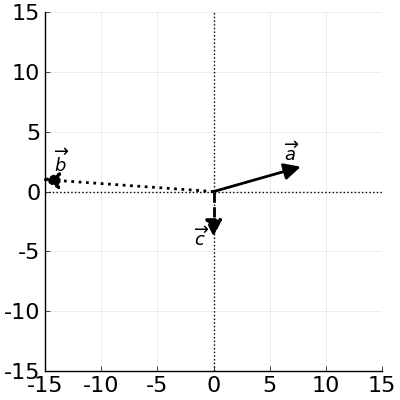
\includegraphics[width=0.44\textwidth]{stretchSquishOp.png}
\caption[.]{The transformations under the linear operator 
{\scriptsize $\begin{bmatrix} 2\frac{1}{2} & 0 \\ 0 & \frac{1}{2} \\
\end{bmatrix}$,} which is a bit like being simultaneously sat on by two
mirror-image hippos.}
\label{fig:stretchSquishOp}
\end{figure}
\index{hippo butts}

\index{squishing}
\index{smooshing}

Figure~\ref{fig:stretchSquishOp} (p.~\pageref{fig:stretchSquishOp}) shows the
results. Our vectors have been both stretched and squished: stretched wide away
horizontally from the $y$-axis, and squished towards the $x$-axis. It's like a
hippo sat down on the $x$-axis -- and his evil twin hippo below him sat ``up''
on the $x$-axis, so that their butts nearly met in the middle. All the blades
of grass on both sides of the axis were smooshed under the composite load.
(Btw, if this visual image isn't doing it for you, by all means disregard it.)

\bigskip

\label{flipOperator}

Okay, now some other things than squishing and stretching. Let's investigate
this smooth operator:

\vspace{-.15in}
\begin{align*}
F_{h} =
\begin{bmatrix}
-1 & 0 \\
0 & 1 \\
\end{bmatrix}.
\end{align*}
\vspace{-.15in}

Almost the same as the identity matrix, except for that minus sign. What does
it do?

\vspace{-.15in}
\begin{align*}
F_{h} \cdot \overrightarrow{\textbf{a}} &=
\begin{bmatrix}
-1 & 0 \\
0 & 1 \\
\end{bmatrix} \cdot
\begin{bmatrix}
3 \\ 4 \\
\end{bmatrix} =
\begin{bmatrix}
-3 \\ 4 \\
\end{bmatrix},
\end{align*}

\vspace{-.15in}
\begin{align*}
F_{h} \cdot \overrightarrow{\textbf{b}} &=
\begin{bmatrix}
-1 & 0 \\
0 & 1 \\
\end{bmatrix} \cdot
\begin{bmatrix}
-6 \\ 2 \\
\end{bmatrix} =
\begin{bmatrix}
6 \\ 2 \\
\end{bmatrix}.
\end{align*}

\vspace{-.15in}
\begin{align*}
F_{h} \cdot \overrightarrow{\textbf{c}} &=
\begin{bmatrix}
-1 & 0 \\
0 & 1 \\
\end{bmatrix} \cdot
\begin{bmatrix}
0 \\ -7 \\
\end{bmatrix} =
\begin{bmatrix}
0 \\ -7 \\
\end{bmatrix}.
\end{align*}
\vspace{-.15in}

As you can see in Figure~\ref{fig:horizFlipOp}, the effect of this operator is
to flip the vectors horizontally through the $y$ axis, like a mirror. A similar
effect can be seen in Figure~\ref{fig:vertFlipOp}, which shows the operator
$F_v$ = {\scriptsize $\begin{bmatrix} 1 & 0 \\ 0 & -1 \\ \end{bmatrix}$}
flipping the picture vertically, through the $x$ axis.

\begin{figure}[ht]
\centering
\vspace{.2in}
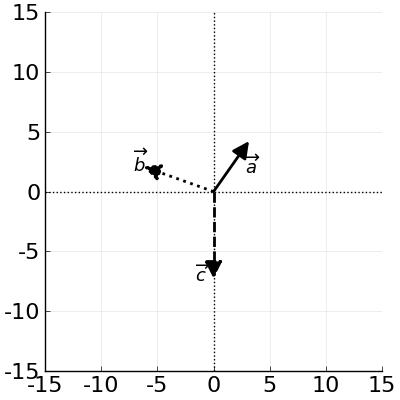
\includegraphics[width=0.44\textwidth]{preoperators.png}
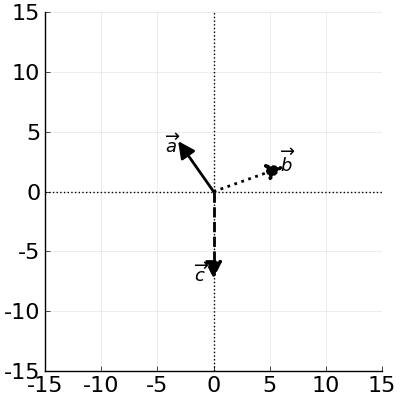
\includegraphics[width=0.44\textwidth]{horizFlipOp.png}
\caption[.]{The action of the linear operator 
{\scriptsize $\begin{bmatrix} -1 & 0 \\ 0 & 1 \\
\end{bmatrix}$,} which flips everything mirror-image wise across the $y$-axis.
To the $\overrightarrow{\textbf{c}}$ vector, this was pretty underwhelming.}
\label{fig:horizFlipOp}
\end{figure}

\begin{figure}[hb]
\centering
\vspace{.2in}
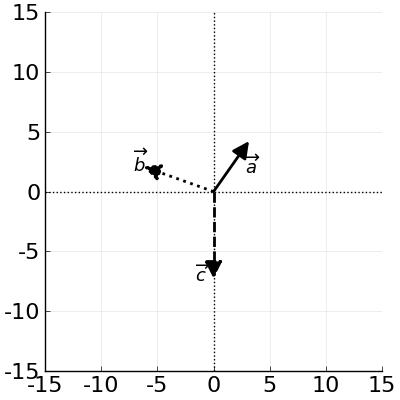
\includegraphics[width=0.44\textwidth]{preoperators.png}
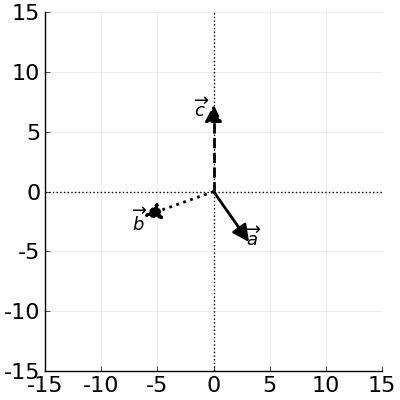
\includegraphics[width=0.44\textwidth]{vertFlipOp.png}
\caption[.]{The action of the linear operator 
{\scriptsize $\begin{bmatrix} 1 & 0 \\ 0 & -1 \\
\end{bmatrix}$,} which flips everything mirror-image wise across the $x$-axis.}
\label{fig:vertFlipOp}
\end{figure}

\medskip

Okay, now my favorite ones. Check out this bad boy:

\vspace{-.15in}
\begin{align*}
R_{+90\degree} =
\begin{bmatrix}
0 & -1 \\
1 & 0 \\
\end{bmatrix}.
\end{align*}
\vspace{-.15in}

Can you guess why I named it the way I did? Check out its operation, and the
resulting graph:

\vspace{-.15in}
\begin{align*}
R_{+90\degree} \cdot \overrightarrow{\textbf{a}} &=
\begin{bmatrix}
0 & -1 \\
1 & 0 \\
\end{bmatrix} \cdot
\begin{bmatrix}
3 \\ 4 \\
\end{bmatrix} =
\begin{bmatrix}
-4 \\ 3 \\
\end{bmatrix},
\end{align*}

\vspace{-.15in}
\begin{align*}
R_{+90\degree} \cdot \overrightarrow{\textbf{b}} &=
\begin{bmatrix}
0 & -1 \\
1 & 0 \\
\end{bmatrix} \cdot
\begin{bmatrix}
-6 \\ 2 \\
\end{bmatrix} =
\begin{bmatrix}
-2 \\ -6 \\
\end{bmatrix}.
\end{align*}

\vspace{-.15in}
\begin{align*}
R_{+90\degree} \cdot \overrightarrow{\textbf{c}} &=
\begin{bmatrix}
0 & -1 \\
1 & 0 \\
\end{bmatrix} \cdot
\begin{bmatrix}
0 \\ -7 \\
\end{bmatrix} =
\begin{bmatrix}
7 \\ 0 \\
\end{bmatrix}.
\end{align*}
\vspace{-.15in}


It \textit{rotates} the vectors 90\textdegree\ counter-clockwise. Neato!

\begin{figure}[ht]
\centering
\vspace{.2in}
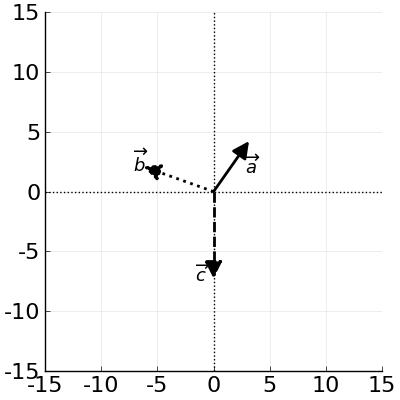
\includegraphics[width=0.44\textwidth]{preoperators.png}
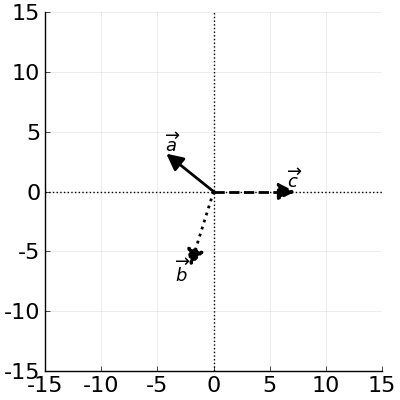
\includegraphics[width=0.44\textwidth]{rotate90op.png}
\caption[.]{The linear operator 
{\scriptsize $\begin{bmatrix} 0 & -1 \\ 1 & 0 \\
\end{bmatrix}$,} which rotates them 90\textdegree\ counter-clockwise.}
\label{fig:rotate90op}
\end{figure}

\index{rotation matrix}

As a matter of fact, we can create a linear operator to rotate vectors
\textit{any} angle we want. Suppose we want to rotate them 63.4\textdegree\ 
counter-clockwise (just to pick a random number). The formula for computing the
rotation matrix is:

\vspace{-.15in}
\begin{align*}
R_{\theta} =
\begin{bmatrix}
\cos \theta & -\sin \theta \\
\sin \theta & \cos \theta \\
\end{bmatrix},
\end{align*}
\vspace{-.15in}

where $\theta$ is the angle we wish to rotate. We plug in $\theta =
63.4\degree$ to get:

\vspace{-.15in}
\begin{align*}
R_{+63.4\degree} =
\begin{bmatrix}
.4478 & -.8942 \\
.8942 & .4478 \\
\end{bmatrix}.
\end{align*}
\vspace{-.2in}

Applying this linear operator to our three vectors, we get these results and
the picture in Figure~\ref{fig:rotate634op}.

\vspace{-.2in}
\begin{align*}
R_{+63.4\degree} \cdot \overrightarrow{\textbf{a}} &=
\begin{bmatrix}
.4478 & -.8942 \\
.8942 & .4478 \\
\end{bmatrix} \cdot
\begin{bmatrix}
3 \\ 4 \\
\end{bmatrix} =
\begin{bmatrix}
-2.2334 \\ 4.4738 \\
\end{bmatrix},
\end{align*}

\vspace{-.2in}
\begin{align*}
R_{+63.4\degree} \cdot \overrightarrow{\textbf{b}} &=
\begin{bmatrix}
.4478 & -.8942 \\
.8942 & .4478 \\
\end{bmatrix} \cdot
\begin{bmatrix}
-6 \\ 2 \\
\end{bmatrix} =
\begin{bmatrix}
-4.4752 \\ -4.4696 \\
\end{bmatrix}.
\end{align*}

\vspace{-.2in}
\begin{align*}
R_{+63.4\degree} \cdot \overrightarrow{\textbf{c}} &=
\begin{bmatrix}
.4478 & -.8942 \\
.8942 & .4478 \\
\end{bmatrix} \cdot
\begin{bmatrix}
0 \\ -7 \\
\end{bmatrix} =
\begin{bmatrix}
6.2594 \\ -3.1346 \\
\end{bmatrix}.
\end{align*}

\begin{figure}[hb]
\centering
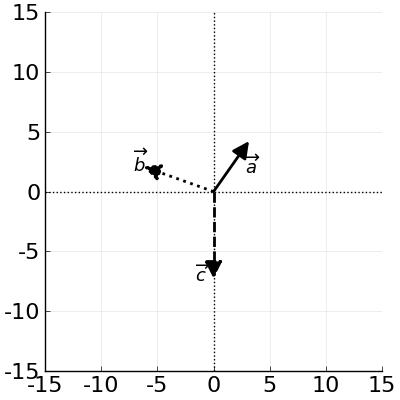
\includegraphics[width=0.40\textwidth]{preoperators.png}
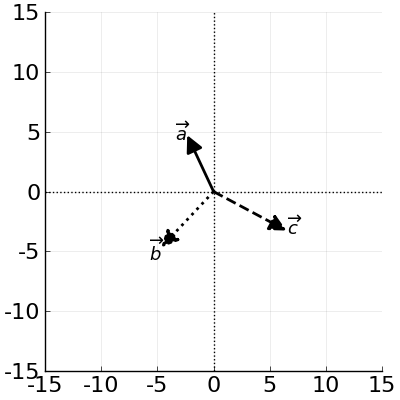
\includegraphics[width=0.40\textwidth]{rotate634op.png}
\caption[.]{The vectors under rotation by 63.4\textdegree\ CCW.}
\label{fig:rotate634op}
\end{figure}

\bigskip

\index{Mario Kart}
\index{CGI movie effects}

I think you get the idea. Linear operators are simple matrices that can perform
a variety of transformative effects on vectors. They're especially helpful (and
easy to visualize) in graphics settings. Every time your Mario Kart character
turns slightly, and sees a different angle of the race track, all of the
scenery and opposing racers have to be drawn in exactly the right places. This
can involve shrinkage, stretching, skewing, rotation, and a variety of other
effects, all of which boil down to linear algebra operations. The same could be
said for CGI movie effects.

\index{Battlestar Galactica}
\index{Thrace, Lt.~Kara}
\index{Starbuck}
\index{colonial viper}
\index{Cylon}

Many people are surprised to learn that underneath the breathtaking scenery and
fist-clenching action sequences of movies and games is a bunch of math.
Watching Lt.~Kara Thrace's viper arc towards the Cylon Resurrection ship seems
like the least ``mathy'' thing in the world: it's all art and images and
motion. But the reason it looks cool (and ``correct'' to the viewer, who has
seen many objects move around in the world before) is that the linear algebra
operations that govern movement and perspective are calculated properly. Truly,
there's nothing cool without math.



\section{The kernel}

\index{kernel}
\index{nullspace}

One curious-sounding mathematical term is ``\textbf{kernel},'' which is a
property of linear operators (and therefore, square matrices). Another word for
a matrix's kernel is its \textbf{nullspace}, which means the same thing.

\index{zero vector}

The kernel of a linear operator is simply this: \textit{the set of input
vectors that it maps to the zero vector.} (A \textbf{zero vector} is just a
vector with all zeroes in it.) Recall that a linear operator acts on vectors of
a particular dimension to produce other vectors of the same dimension. What's
under consideration here is: ``what can we feed in to this operator and get all
zeroes?'' That may not seem like a very interesting question, but it turns out
to be.

Let's start with an example. On p.~\pageref{flipOperator} we had this linear
operator:

\vspace{-.15in}
\begin{align*}
F_{h} =
\begin{bmatrix}
-1 & 0 \\
0 & 1 \\
\end{bmatrix},
\end{align*}
\vspace{-.15in}

whose function, when we worked it out, was to flip vectors horizontally through
the $y$-axis. The vector $[\ 2\ \ 3\ ]$ was transformed to $[\ -2\ \ 3\ ]$; the
vector $[\ -4\ \ -1\ ]$ was mapped to $[\ 4\ \ -1\ ]$; and the like. Each input
was mapped to its mirror image.

Now consider the kernel question. What is the complete set of vectors which,
when subjected to the operation of $F_{h}$, would turn into $[\ 0\ \ 0\ ]$. I
think you'll see in a moment's thought that there is only one such vector;
namely, $[\ 0\ \ 0\ ]$ itself. Only if you're already \textit{on} the origin is
your mirror image in the $y$-axis also going to be the origin. Hence, the
kernel of $F_{h}$ is only the zero vector. Notationally, we write:

\vspace{-.15in}
\begin{align*}
\ker F_{h} = \{ 
\begin{bmatrix}
0 \\ 0 \\
\end{bmatrix}
\}.
\end{align*}
\vspace{-.15in}

\index{set}
\index{origin}

The word ``ker'' stands for kernel, of course, and since we defined an
operator's kernel as the \textit{set} of vectors that get mapped to the zero
vector, we put our one and only kernel vector in curly braces to designate
that.

\index{trivial@``trivial'' solution}
Now do you remember way back on p.~\pageref{trivialSolution} when we spoke of
the ``trivial solution'' of a pair of dominoes? You might want to flip back to
that page and refresh your memory. The subject under discussion was how to get
to the \textit{origin} via a linear transformation of a set of dominoes. In
true Domino Game fashion, you could add any multiple of the first domino to any
multiple of the second, and in this case the goal was to get the domino
\raisebox{-0.25\height}{
\includegraphics[width=0.07\textwidth]{white0_0.png}}.
The conclusion we came to was that if the dominoes were \textit{yellow}
(\textit{i.e.}, if they were linearly independent of one another) there was no
way to get to the origin except by, duh, taking zero of the first domino and
zero of the second.

You should immediately see the tie-in with the kernel concept. Since every
matrix-vector multiplication is a linear combination of the matrix's columns
(interpretation 2 on p.~\pageref{twoInterpretations}), asking what vectors get
mapped to the zero vector is the same as asking what linear combinations take
you to the origin. And the fact of the matter is that if your matrix has
linearly independent columns (yellow dominoes) then there is only one such
linear combination: zero of the first, and zero of the second.

\smallskip

What about our rotation matrix?

\vspace{-.15in}
\begin{align*}
R_{+90\degree} =
\begin{bmatrix}
0 & -1 \\
1 & 0 \\
\end{bmatrix}.
\end{align*}
\vspace{-.15in}

\index{rotation matrix}
\index{whirlpool}

Again, visualizing it geometrically tells you the answer. Every point is
rotated 90\textdegree\ counter-clockwise about the origin. So the only way to
\textit{land} in the middle of the whirlpool is to \textit{start} in the middle
of the whirlpool. Again, we have just the zero vector: $\ker R_{+90\degree} = \{
{\scriptsize \begin{bmatrix} 0 \\ 0
\\ \end{bmatrix}} \}$.

\smallskip

What about our squishing/stretching matrices, like this one:

\vspace{-.15in}
\begin{align*}
S_{v=\frac{1}{2},h=2\frac{1}{2}} =
\begin{bmatrix}
2\frac{1}{2} & 0 \\
0 & \frac{1}{2} \\
\end{bmatrix}?
\end{align*}
\vspace{-.15in}

\index{squishing}
\index{smooshing}
\index{stretching}

Same thing. Every point will be (1) moved halfway closer to the $x$-axis than
it was, and (2) moved two-and-a-half times further from the $y$-axis than it
was. So the only way to land on the origin is to start on the origin, and once
again we have $\ker S_{v=\frac{1}{2},h=2\frac{1}{2}} = \{ {\scriptsize
\begin{bmatrix} 0 \\ 0 \\ \end{bmatrix}} \}$.

\bigskip

You're probably starting to wonder whether this is always the case. Does
\textit{any} linear operator have a bigger kernel?

But the answer, as you may remember from p.~\pageref{trivialSolution}, is
\textbf{yes}: if our columns are \textit{blue dominoes}. Linearly
\textit{de}pendent vectors makes it so that there are many ways to get to the
origin.

Let's try a linear operator with blue domino columns, like this one:

\vspace{-.15in}
\begin{align*}
B =
\begin{bmatrix}
\frac{1}{2} & 1 \\
-1 & -2 \\
\end{bmatrix}.
\end{align*}
\vspace{-.15in}

First, convince yourself that the columns are indeed linearly independent. If
you took the left column, $[\ \frac{1}{2} \ \ -1\ ]$, and you multiplied that
column by 2, you would get $[\ 1\ \ -2\ ]$, which is the right column. So yes,
they are.

\begin{figure}[ht]
\centering
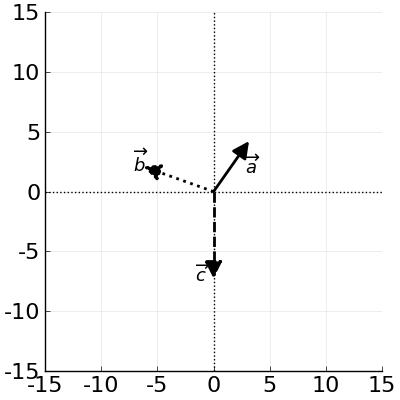
\includegraphics[width=0.40\textwidth]{preoperators.png}
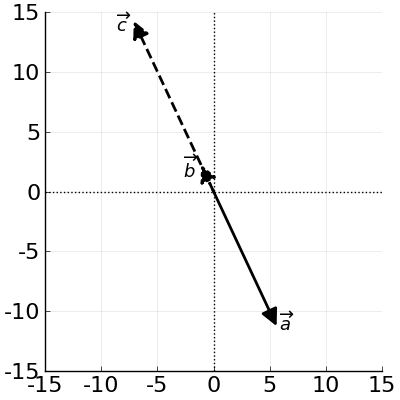
\includegraphics[width=0.40\textwidth]{bluedominoesop.png}
\caption[.]{The vectors transformed by an operator $B$ whose columns are
linearly dependent.}
\label{fig:bluedominoesop}
\end{figure}

The effect, shown in Figure~\ref{fig:bluedominoesop}, is rather jarring. This
narrow-minded matrix slapped all three vectors down in exactly the same
direction! This is because just as blue dominoes can only move you on a certain
line of the two-dimensional plane, so \textit{they can only map input vectors
to that line}.

\index{trivial@``trivial'' solution}

Now the ``good news'' (if you call it that) for blue dominoes is that there is
indeed more than one way to get to the origin by using them -- more than just
the ``trivial solution.'' And this in turn means that the \textit{kernel} is
larger than just the zero vector. Just check out all these vectors that get
mapped to the origin:

\vspace{-.15in}
\begin{align*}
\small
\textrm{the vector }
{\scriptsize
\begin{bmatrix}
-2 \\ 1 \\
\end{bmatrix}}: \quad
\begin{bmatrix}
\frac{1}{2} & 1 \\
-1 & -2 \\
\end{bmatrix} \cdot
\begin{bmatrix}
-2 \\ 1 \\
\end{bmatrix} &=
\begin{bmatrix}
0 \\ 0 \\
\end{bmatrix}
\checkmark \\
\textrm{the vector }
{\scriptsize
\begin{bmatrix}
-4 \\ 2 \\
\end{bmatrix}}: \quad
\begin{bmatrix}
\frac{1}{2} & 1 \\
-1 & -2 \\
\end{bmatrix} \cdot
\begin{bmatrix}
-4 \\ 2 \\
\end{bmatrix} &=
\begin{bmatrix}
0 \\ 0 \\
\end{bmatrix}
\checkmark \\
\textrm{the vector }
{\scriptsize
\begin{bmatrix}
6 \\ -3 \\
\end{bmatrix}}: \quad
\begin{bmatrix}
\frac{1}{2} & 1 \\
-1 & -2 \\
\end{bmatrix} \cdot
\begin{bmatrix}
6 \\ -3 \\
\end{bmatrix} &=
\begin{bmatrix}
0 \\ 0 \\
\end{bmatrix}
\checkmark \\
\textrm{the vector }
{\scriptsize
\begin{bmatrix}
67 \\ -33\frac{1}{2} \\
\end{bmatrix}}: \quad
\begin{bmatrix}
\frac{1}{2} & 1 \\
-1 & -2 \\
\end{bmatrix} \cdot
\begin{bmatrix}
67 \\ -33\frac{1}{2} \\
\end{bmatrix} &=
\begin{bmatrix}
0 \\ 0 \\
\end{bmatrix}
\checkmark \\
\textrm{the vector }
{\scriptsize
\begin{bmatrix}
-\frac{1}{9} \\ \frac{1}{18} \\
\end{bmatrix}}: \quad
\begin{bmatrix}
\frac{1}{2} & 1 \\
-1 & -2 \\
\end{bmatrix} \cdot
\begin{bmatrix}
-\frac{1}{9} \\ \frac{1}{18} \\
\end{bmatrix} &=
\begin{bmatrix}
0 \\ 0 \\
\end{bmatrix}
\checkmark \\
\end{align*}
\normalsize
\vspace{-.15in}

So at this point, we've discovered that the kernel of $B$ has \textit{at least}
these vectors in it:

\vspace{-.15in}
\begin{align*}
\ker B =
\small
\{
\begin{bmatrix}
-2 \\ 1 \\
\end{bmatrix}, 
\begin{bmatrix}
-4 \\ 2 \\
\end{bmatrix}, 
\begin{bmatrix}
6 \\ -3 \\
\end{bmatrix}, 
\begin{bmatrix}
67 \\ -33\frac{1}{2} \\
\end{bmatrix}, 
\begin{bmatrix}
-\frac{1}{9} \\ \frac{1}{18} \\
\end{bmatrix}, \cdots \} \\
\end{align*}
\normalsize
\vspace{-.15in}

Now the shrewd reader will notice something interesting about all those vectors
in the kernel. Can you spot the pattern?

It's actually pretty simple. Whatever number you choose for the first element
of the vector, the second element has to be negative-half-of that. The first
example, $[\ -2\ \ 1\ ]$, has $-2$ in the first element, and
negative-half-of-that (which is 1) as its second element. Similarly, 2 is
negative-half-of $-4$, $-3$ is negative-half-of 6, and so forth.

\index{degree of freedom}

Now a subtle but important fact here is that our ``choice process'' for finding
vectors in $\ker B$ has \textit{one degree of freedom} to it. We're free to
choose whatever we like for one of the vector's elements. But then, if we want
the vector to be in the kernel of $B$, we have no flexibility in what we choose
for the other. Our only choice is to divide it by 2 and change its
sign. Any other choice for that second element won't result in a vector that
maps to ${\scriptsize \begin{bmatrix} 0 \\ 0 \end{bmatrix}}$.

We could express this in symbols by saying that you get one variable -- call it
$x$ -- for your free choice, at which point you can declare this vector to be
in $B$'s kernel:

\vspace{-.15in}
\begin{align*}
\begin{bmatrix}
x \\ -\frac{x}{2} \\
\end{bmatrix}.
\end{align*}
\vspace{-.15in}

If you're a visual person, you can let $x$ freely range from $-\infty$ to
$\infty$, and plot this vector for all possible values of $x$ plugged in. Your
plot would look like Figure~\ref{fig:nullspace1}: a one-dimensional straight
line.

\begin{figure}[ht]
\centering
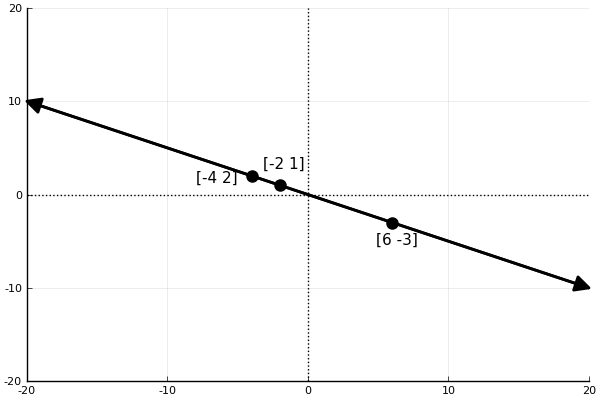
\includegraphics[width=0.8\textwidth]{nullspace1.png}
\caption[.]{The kernel (nullspace) of $B$, plotted visually. Any vector whose
tip lies on that straight line will be in $\ker B$, which means we have a
one-dimensional kernel.}
\label{fig:nullspace1}
\end{figure}

\section{Nullity}

Okay, so with $B$, we had one degree of freedom in constructing a vector in the
kernel. Now with our other linear operators from this chapter -- like $F_{h}$,
$R_{63.4\degree}$, and friends -- we actually had \textit{zero} degrees of
freedom! There simply weren't any free choices to make at all: we simply had to
say ``uh, the only vector in the kernel is ${\scriptsize \begin{bmatrix} 0 \\ 0
\end{bmatrix}}$ itself. Nothin' much we can do about that.''

\index{dimension}
\index{nullity}
\index{kernel}

With that prelude out of the way, it's time for a new term. The
\textbf{nullity} of a linear operator (square matrix) is \textit{the dimension
of its kernel}. The idea of ``dimension'' here is closely linked to the concept
of ``degrees of freedom.'' In Figure~\ref{fig:nullspace1}, you can see that all
the points in $B$'s kernel are lined up on a straight line. A line is a
\textit{one}-dimensional shape: you can specify any point on it with just one
coordinate, telling you how far leftwards or rightwards you are. Hence the
dimension of $B$'s kernel -- or its ``nullity'' -- is 1.

A mere point, on the other hand, is a \textit{zero}-dimensional shape: there's
nothing to specify further about it -- it's just a point, man. So what this
means is that in a $2\times 2$ matrix with linearly \textit{in}dependent
columns -- like $F_{h}$, or $S_{v=\frac{1}{2},h=2\frac{1}{2}}$, or even the
identity matrix $I$ -- \textit{the \textbf{nullity} is 0}. Only if the matrix
has linearly \textit{de}pendent columns, will its nullity will be greater than
0. In $B$'s case, it is 1. Sometimes you'll see the notation:

\vspace{-.15in}
\begin{center}
null $B$ = 1
\end{center}
\vspace{-.15in}

which means ``the nullity of the $B$ operator is 1, which in turn means there's
one degree of freedom you get in constructing a vector that will wind up in
$B$'s kernel.''

\section{Rank}
\index{rank}
\index{full-rank matrix}

This in turn is related to yet another new term: the \textbf{rank} of a matrix.
A square matrix's rank is \textit{the number of linearly independent columns it
has.} That's a relatively simple idea. If I give you a $3\times 3$ matrix, you
know the rank can't be possibly greater than 3, because there are only three
columns in it, \textit{period.} The question, then, is how many of those
columns can be arrived at by linear combinations of the others? If none of them
can, then you have a fully healthy yellow domino matrix with three fresh
columns that each point in totally different directions. It's a rank 3 matrix.
Since it's rank 3 and there are three total columns, it's also sometimes called
a \textbf{full-rank} matrix.

\index{rank-deficient}

On the other hand, if some of those columns are linearly dependent on others,
then we're in a blue domino situation. Suppose you can get the third column
from a linear combination of the other two, but that the first two are indeed
independent with respect to each other. Then, we have a rank 2 matrix: it's
``one card short of a full deck,'' as they say. Another term for a matrix whose
rank is less than its number of columns is a \textbf{rank-deficient} matrix,
for obvious reasons.

\section{The Rank-Nullity Theorem}

And now we can wrap this chapter up with a bow. It turns out that the concepts
of rank and nullity are intimately bound up together, and in a very simple way;
namely,

\vspace{-.15in}
\begin{center}
rank $A$ + null $A$ = number of columns of $A$,
\end{center}
\vspace{-.15in}

\index{rank-nullity theorem}

for any square matrix $A$. This is called the \textbf{rank-nullity theorem},
and you can take it to the bank.

Let's think about what it means. If you just grab a random square matrix off
the shelf at Wal-Mart, it's going to be full rank. If you grab a $3\times 3$
matrix, you'd have to have awful bad luck for one of the columns to be an exact
linear combination of the two others. In this case, then, it'll be a full-rank
matrix; or put another way, its rank will be 3. And as we've seen in the above
examples, the only vector it will map to the origin will be the zero vector
itself. That's a zero-dimensional ``space,'' and hence the nullity is 0. And so
the formula holds: a rank of 3, plus a nullity of 0, equals 3 columns in our
matrix.

If we're unlucky, and we get one column being linearly dependent on the other
two, then we have a rank-deficient matrix with blue columns. Since only two of
the columns are really ``legit,'' it's a rank 2 matrix. And from the previous
analysis, we've seen that such matrices have an entire line in their kernel,
not just one point. That one-dimensional line means that their nullity is 1.
And again for formula holds: a rank of 2, plus a nullity of 1, equals 3 columns
in our matrix.

It turns out some $3\times 3$ matrices are even suckier than that. Suppose we
get one that has only \textit{one} linearly independent column -- each of the
other two are exact (possibly scaled) duplicates of the other one! It's not
hard to create such a matrix; how about:

\vspace{-.15in}
\begin{align*}
S =
\begin{bmatrix}
1 & 2 & 3 \\
2 & 4 & 6 \\
3 & 6 & 9 \\
\end{bmatrix}.
\end{align*}
\vspace{-.15in}

\index{sucky matrix}

(``$S$'' stands for ``sucky.'') We scratch our head looking at that guy: sure,
we've been given permission to go in direction $[\ 1\ 2\ 3\ ]$, which is great
and all, but the other two columns just give us regurgitated versions of that.
There's no additional power in being able to travel in the $[\ 2\ 4\ 6\ ]$
direction if you can already go in the $[\ 1\ 2\ 3\ ]$ direction, because
they're the same direction! And the same is true of the last column as well.

In this case, it turns out to be a rank \textit{1} matrix -- only one
independent column. And you'll find that its nullity is therefore \textit{2}.
There's an entire two-dimensional plane (hanging out in three-dimensional space)
any point on which will be in $S$'s kernel. And again, the rank-nullity theorem
holds: a rank of 1 plus a nullity of 2 equals 3 columns in the matrix.

This deep relationship holds in any number of dimensions and even in
non-real-valued matrices. It's a beautifully descriptive way to capture exactly
how much power a matrix has to perform linear transformations.
